\chapter{Area and Volume}
\graphicspath{{foto/Chap4/}}
In this chapter we have computed the area and the volume of the complete structure of the register file (10T Cell, Decoders and Sense Amplifier).

\section{Memory Block}
For the area and volume evaluation of the memory, the model in figure \ref{fig:cube} has been used.

\begin{center}
	\begin{figure}[H]
		\centering
		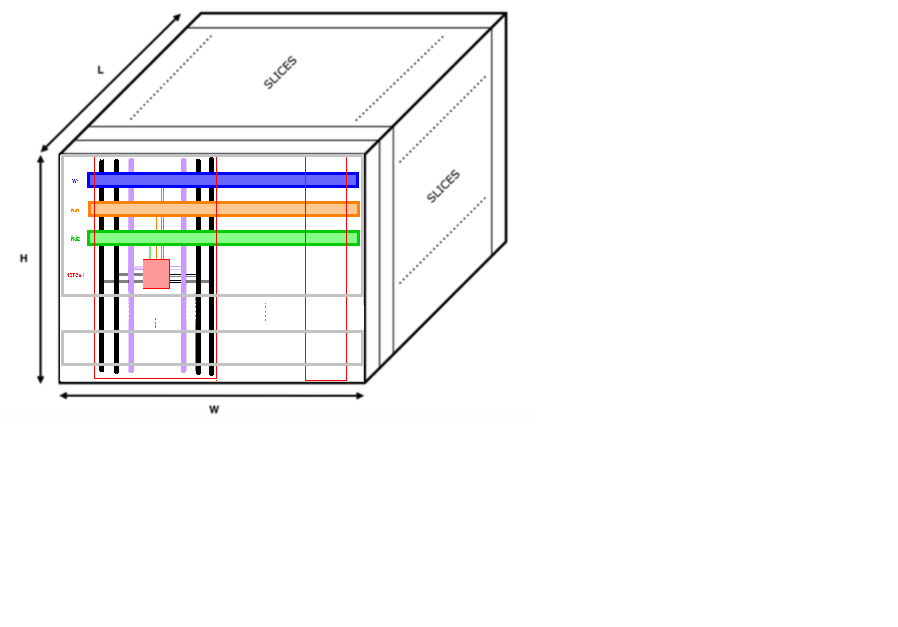
\includegraphics[scale = 0.9, trim={0 5cm 10cm 0},clip]{cube}
		\caption{Simplified Register File structure}
		\label{fig:cube}
	\end{figure}
\end{center}

The three dimensions of the array have been computed as follows:

\begin{itemize}
	\item \textit{Width, Length}: In order to find these values, the area of the elementary bit cell has been calculated and then its square root has been used in order to compute width and length.
	\[
	\textbf{Area\_BitCell}=2 \cdot (N\_port\_Wr+N\_port\_Rd) \cdot Tr\_n\_Area +
	\]
	\[
	+ 2 \cdot (Tr\_n\_Area + Tr\_p\_Area)
	\]
	\[
	\textbf{W}=(2 \cdot (N\_port\_Wr + N\_port\_Rd) \cdot Pitch_{pp} + \sqrt{Area\_BitCell}) \cdot N_{bit} +
	\]
	\[
	+ Pitch_{pp} \cdot (N_{bit}-1)
	\]
	\[
	\textbf{L}=N_{block} \cdot Pitch_{pp}
	\]
	
	As it can be seen, the area of the SRAM memory cell is computed as function of the number of read and write ports. Other elements, influenced by the number of input ports, are the number of wordline and bitline: this will affect the width and, as it can be seen in the following step, the height of the memory block.
	
	\item \textit{Height of the stack}: the terms considered are the height of the Cells that takes into account of the the number of Read and Write lines and their distances, the square root of the Area of bit cells, and the distance between them, as shown in \ref{fig:Stack}.
	\[
	\textbf{H}=((N\_port\_Wr+N\_port\_Rd) \cdot Pitch_{pp} + \sqrt{Area\_BitCell}) \cdot N_{bit} +
	\]
	\[
	+ Pitch_{pp} \cdot (N_{bit}-1)	
	\]
	
Finally, the area and the volume of the Register File can be calculated as:
	\[
	\textbf{Memory\_Array\_Area}=H \cdot W
	\]
	\[
	\textbf{Memory\_Array\_Volume}=H \cdot W \cdot L
	\]
	
\begin{center}
	\begin{figure}[H]
		\centering
		\includegraphics[scale = 0.4]{section_pillars}
		\caption{Stack structure}
		\label{fig:Stack}
	\end{figure}
\end{center}
\end{itemize}

\section{Decoders}
For the area and volume evaluation of all the decoders, the model that has been used is the same described in the Chapter 2. For each decoder the number of n-type transistors was first calculated and then the number of p-type transistors; subsequently they have been multiplied by their minimum area value and then added together to calculate the total area. Finally the volume has been calculated as the multiplication of the Area and the length.

\begin{itemize}
\item{\textbf{Block Decoder}}:
The area of the \textit{Block Decoder} has been calculated as: area of the the core of the decoder added to the area of the inverter connected at the input and and at the output. In this case the number of input is given by the \textit{Block Address} while the output is equal to the number of slice $N_{slice}$. The volume is the area multiplied by the single distance between two transistor because there is only one \textit{Block Decoder}. So:
	\[
	\#Tr\_n\_Block\_Dec = Block\_Address \cdot N_{slice} + N_{slice} + Block\_Address
	\]
	\[
	\#Tr\_p\_Block\_Dec = 2 \cdot N_{slice} + Block\_Address
	\]
	\\
	\[
	\textbf{Block\_Dec\_Area} = \#Tr\_n\_Block\_Dec \cdot Tr\_n\_Area +
	\]
	\[
	+ \#Tr\_p\_Block\_Dec \cdot Tr\_p\_Area
	\]
	\[
	\textbf{Block\_Dec\_Volume} = Block\_Dec\_Area \cdot Pitch_{pp}
	\]

\item{\textbf{Row Decoder}}:
The area of the \textit{Row Decoder} has been calculated as before but in this case the number of input is done by the \textit{Row Address} while the output is equal to the number of row that is $(N_{wl})$. This is finally multiplied by the total number of read and write ports. The volume is the area multiplied by the length. So:
	\[
	\#Tr\_n\_Row\_Dec = Row\_Address \cdot N_{wl} + N_{wl} + Row\_Address
	\]
	\[
	\#Tr\_p\_Row\_Dec = 2 \cdot N_{wl} + Row\_Address
	\]
	\\
	\[
	\textbf{Row\_Dec\_Area} = (N\_port\_Wr+N\_port\_Rd) \cdot (\#Tr\_n\_Row\_Dec \cdot Tr\_n\_Area +
	\]
	\[
	+ \#Tr\_p\_Row\_Dec \cdot Tr\_p\_Area)
	\]
	\[
	\textbf{Row\_Dec\_Volume} = Row\_Dec\_Area \cdot L
	\]
\newpage

\item{\textbf{Decoder Address}}:
The previous variables $Block\_Address$, $Row\_Address$,\\ $N\_wl$ and $N\_block$ are computed as:

	\[
	Block\_Address = ceil(log_{2}(N_{block}))
	\]
	\[
	Row\_Address = ceil(log_{2}(N_{wl}))
	\]
	\[
	N\_wl=min(N\_word,N\_bit)
	\]
	\[
	N\_block = ceil \Bigl ( \frac{N\_word} {N\_bit}\Bigl )
	\]

\end{itemize}
\section{Bit Line Inverters, Pass Transistors \\and Precharge Transistors}
In the total structure there are some pass transistor of n-type used to help the selection of the wanted memory cell.
\begin{itemize}
\item{\textbf{Bit Line Inverters}}:
The area has been calculated as $N_{bl}$ multiplied by the area of single p-type and n-type transistor p-type and n-type and then multiplied by the total number of read and write ports, while the volume is the area multiplied by the length. So:
	\[
	\textbf{Inverter\_bl\_Area} = (N\_port\_Wr+N\_port\_Rd) \cdot \cdot (N_{bl} \cdot Tr\_n\_Area +
	\]
	\[
	+ N_{bl} \cdot Tr\_p\_Area)
	\]
	\[
	\textbf{Inverter\_bl\_Volume} = Inverter\_bl\_Area \cdot L
	\]

\item{\textbf{Row Pass Transistors}}:
The area has been calculated as $N_{wl}$ multiplied by the area of single transistor and then multiplied by the total number of read and write ports, while the volume is the area multiplied by the length. So:
	\[
	\textbf{Pass\_Row\_Area} = (N\_port\_Wr+N\_port\_Rd) \cdot N_{wl} \cdot Tr\_n\_Area
	\]
	\[
	\textbf{Pass\_Row\_Volume} = Pass\_Row\_Area \cdot L
	\]
\item{\textbf{Column Pass Transistors}}:
The area has been calculated as $N_{bl}$ multiplied by the area of single transistor and then multiplied by the total number of read ports, while the volume is the area multiplied by the length. So: 
	\[
	\textbf{Pass\_Column\_Area} = N\_port\_Rd \cdot N_{bl} \cdot Tr\_n\_Area
	\]
	\[
	\textbf{Pass\_Column\_Volume} = Pass\_Column\_Area \cdot L
	\]
\item{\textbf{Slice Pass Transistors}}:
The area is the area of single transistor and then multiplied by the total number of read ports, while the volume is the area multiplied by the length. So:
	\[
	\textbf{Pass\_Slice\_Area} = N\_port\_Rd \cdot Tr\_n\_Area
	\]
	\[
	\textbf{Pass\_Slice\_Volume} = Pass\_Slice\_Area \cdot L
	\]
\item{\textbf{Precharge Transistors}}:
The area has been calculated as $N_{bl}$ multiplied by the area of single p-type transistor and then multiplied by the total number of read ports, while the volume is the area multiplied by the length. So:
	\[
	\textbf{Precharge\_Area} = N\_port\_Rd \cdot N_{bl} \cdot Tr\_p\_Area
	\]
	\[
	\textbf{Precharge\_Volume} = Precharge\_Area \cdot L
	\]
\end{itemize}

\section{Sense Amplifier}
The area of the two \textit{Sense Amplifiers} has been calculated as remembering the structure described in Chapter 2 and the volume is the area multiplied by the length. So:

	\[
	\#Tr\_n\_SA=N_{bl} \cdot 3
	\]
	\[
	\#Tr\_p\_SA=N_{bl} \cdot 3
	\]
	\\
	\[
	\textbf{SA\_Area} = N\_port\_Rd \cdot (\#Tr\_n\_SA \cdot Tr\_n\_Area + \#Tr\_p\_SA \cdot Tr\_p\_Area)
	\]
	\[
	\textbf{SA\_Volume} = SA\_Area \cdot L
	\]

\section{Total Area and Total Volume}
The total area has been calculated has the sum of the area of the memory array and all the boundary circuits:
	\[
	\textbf{Total\_Area}= Memory\_Array\_Area + Block\_Dec\_Area + Row\_Dec\_Area + 
	\]
	\[
	+ Pass\_Row\_Area + Pass\_Column\_Area + Pass\_Slice\_Area +
	\]
	\[
	+ Inverter\_bl\_Area +  SA\_Area
	\]
The total volume has been calculated has the sum of the volume of the memory array and all the boundary circuits:
	\[
	\textbf{Total\_Volume}= Memory\_Array\_Volume + Block\_Dec\_Volume + Row\_Dec\_Volume + 
	\]
	\[
	+ Pass\_Row\_Volume + Pass\_Column\_Volume + Pass\_Slice\_Volume +
	\]
	\[
	+ Inverter\_bl\_Volume +  SA\_Volume
	\]
\section{Simulation result}
In order to verify the the computations made before, it has been made a simulation; in particular it has been reported two graphs in which are represented how the area and the volume change with the only value of $N_{bit}$ since the assumption is that the Register File is a perfect cube. In particular, the array of values it has been considered for $N_{bit}$ is $[8, 16, 32, 64, 128]$.
\\The behaviours represented are reasonable: in the two graphs \ref{fig:1} and \ref{fig:2} there is a square dependency. Changing the value of this parameter, the total area increases quadratically and the volume increase quadratically too.\\
The obtained results are reported in the following figures.

\begin{center}
	\begin{figure}[H]
		\centering
		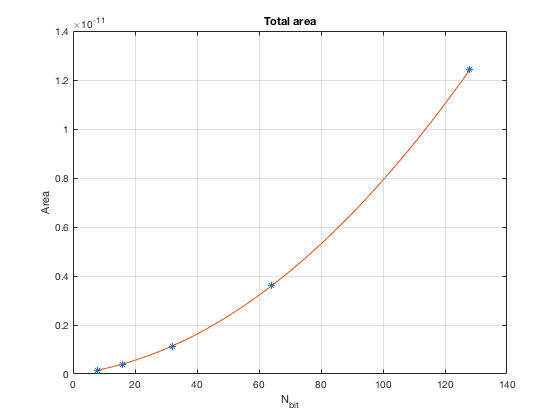
\includegraphics[scale=0.4]{Total_Area.png}
		\caption{Simulation of the Total Area value, varying the number of bit.} 
		\label{fig:1}
	\end{figure}
\end{center}

\begin{center}
	\begin{figure}[H]
		\centering
		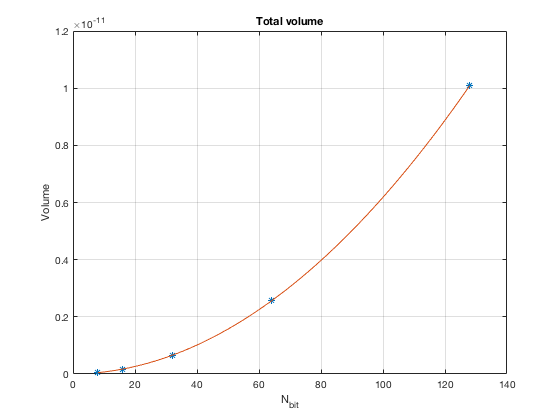
\includegraphics[scale=0.4]{Total_Volume.png}
		\caption{Simulation of the Total Volume value, varying the number of bit.}
		\label{fig:2} 
	\end{figure}
\end{center}

